\newpage
\section{Dùng công cụ Excel, SPSS, Python và R tính toán}

\subsection{Thực hiện One-way ANOVA bằng Excel}

Các bước thực hiện phân tích One-way ANOVA bằng phần mềm Excel được tiến hành như sau:

\begin{enumerate}
\item \textbf{Nhập dữ liệu}

Nhập dữ liệu của ba nhóm vào bảng Excel theo từng cột, mỗi cột tương ứng với một nhóm quan sát (Nhóm 1, Nhóm 2, Nhóm 3).

\item \textbf{Kích hoạt Analysis ToolPak}

Vào \textbf{File $\rightarrow$ Options $\rightarrow$ Add-ins}.  
Tại mục \textit{Excel Add-ins}, chọn \textbf{Analysis ToolPak} và nhấn \textbf{OK} để kích hoạt công cụ phân tích dữ liệu.

\item \textbf{Thực hiện phân tích ANOVA}

\begin{figure}[!htp]
    \centering
    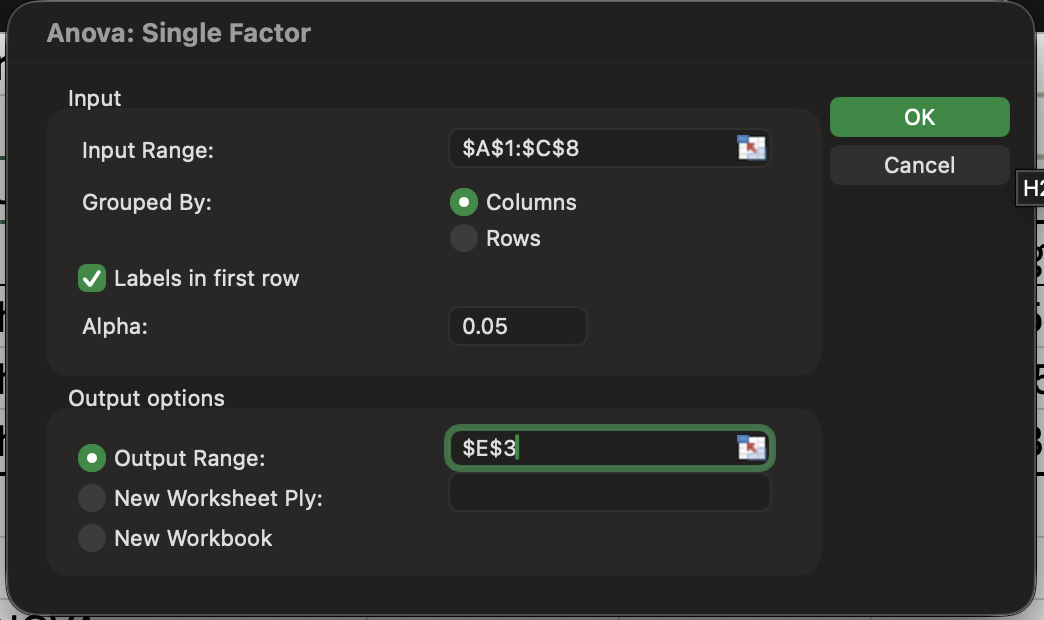
\includegraphics[width=0.6\textwidth]{LAB02/pics/ANOVA_option.png}%
    \caption{Tùy chỉnh khi tính ANOVA trên Excel}
    \label{fig:ANOVA_setup}
\end{figure}

Vào tab \textbf{Data} $\rightarrow$ chọn \textbf{Data Analysis} $\rightarrow$ chọn \textbf{ANOVA: Single Factor}.

Sau đó thiết lập các tham số:
\begin{itemize}
\item \textbf{Input Range}: chọn toàn bộ vùng dữ liệu của ba nhóm.
\item \textbf{Grouped By}: chọn \textbf{Columns}.
\item \textbf{Labels in First Row}: tích chọn nếu có tiêu đề cột.
\item \textbf{Alpha}: nhập giá trị $0.05$.
\item \textbf{Output Range}: chọn vị trí hiển thị kết quả.
\end{itemize}


\item \textbf{Xem kết quả}
\begin{figure}[!htp]
    \centering
    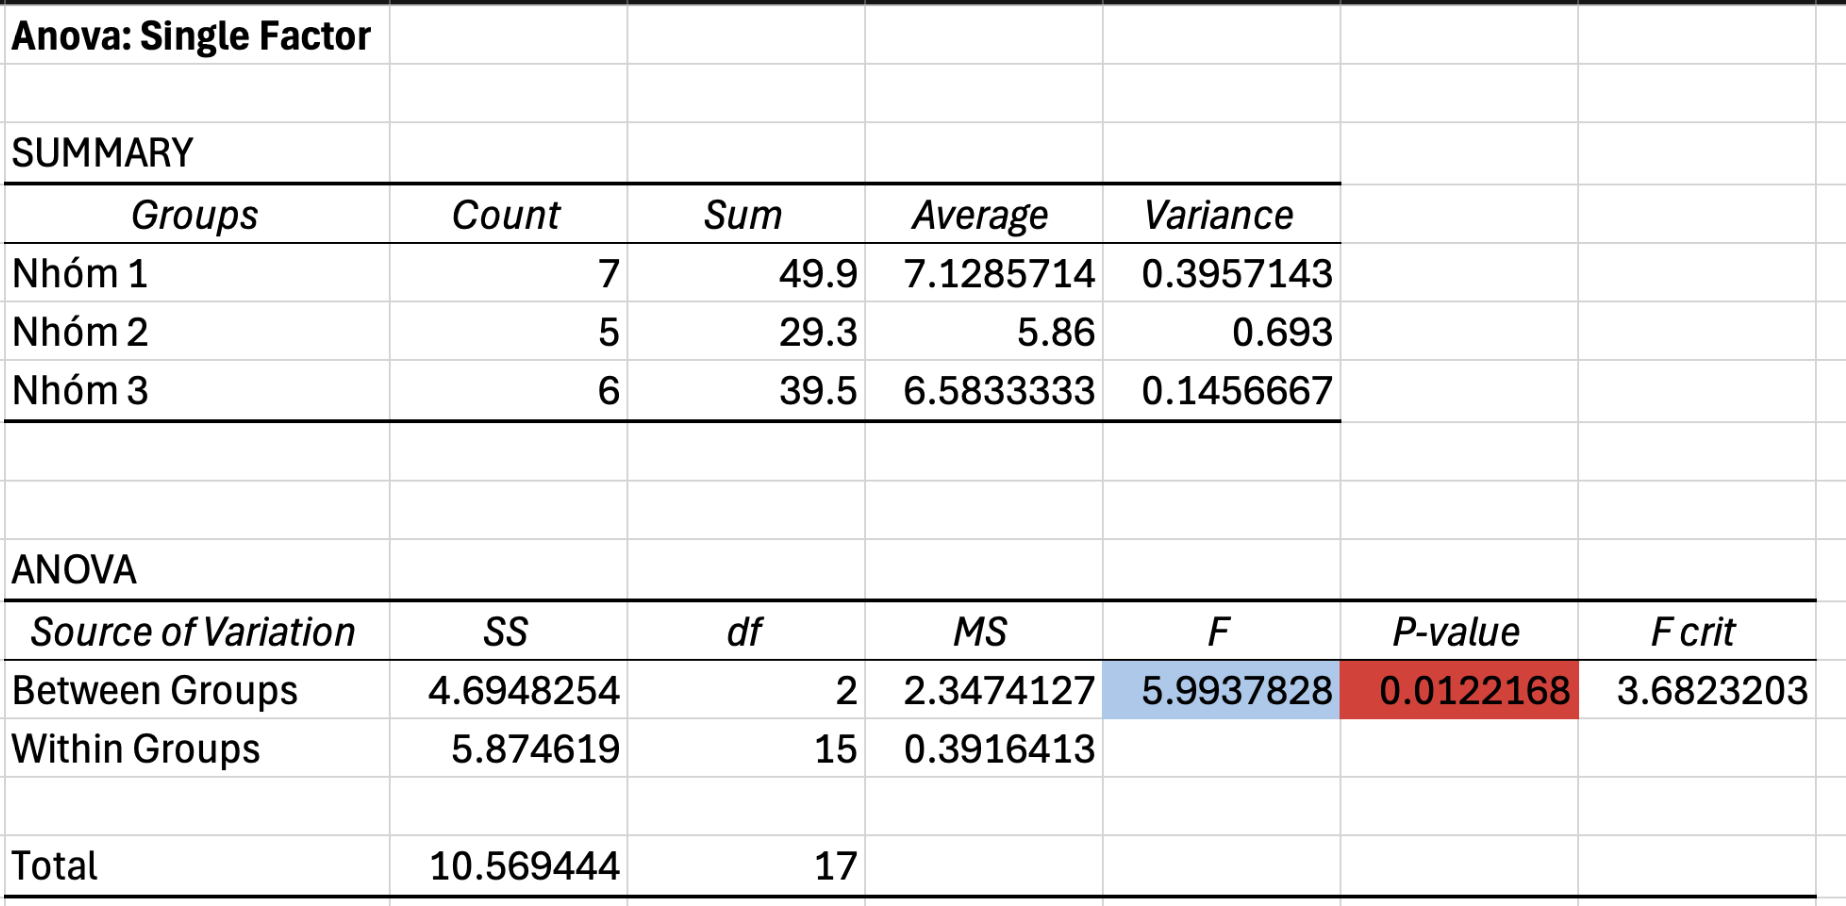
\includegraphics[width=0.6\textwidth]{LAB02/pics/ANOVA_res.png}%
    \caption{Kết quả tính ANOVA: Single Factor từ Excel}
    \label{fig:ANOVA_res}
\end{figure}

Excel sẽ xuất bảng kết quả ANOVA bao gồm các thông tin như:
\begin{itemize}
\item Sum of Squares (SS)
\item Degrees of Freedom (df)
\item Mean Square (MS)
\item F-statistic
\item P-value
\end{itemize}

\item \textbf{Đưa ra kết luận}

So sánh giá trị \textit{P-value} với mức ý nghĩa $\alpha = 0.05$:

\begin{itemize}
\item Nếu $p$-value $< 0.05$ thì bác bỏ giả thuyết $H_0$, kết luận rằng có sự khác biệt trung bình giữa các nhóm.
\item Nếu $p$-value $\ge 0.05$ thì không bác bỏ $H_0$, kết luận rằng chưa có đủ bằng chứng cho thấy sự khác biệt giữa các nhóm.
\end{itemize}
\end{enumerate}

\textbf{Kết luận:}

Từ bảng ANOVA, ta có $p$-value $= 0.0122 < \alpha = 0.05$. Vì vậy, ta bác bỏ giả thuyết $H_0$.

Điều này cho thấy có sự khác biệt có ý nghĩa thống kê giữa giá trị trung bình của ít nhất một trong ba nhóm. Do đó, cần tiếp tục thực hiện kiểm định hậu nghiệm Tukey HSD để xác định cụ thể cặp nhóm nào có sự khác biệt.

\subsection{Kiểm định hậu nghiệm Tukey HSD}

Sau khi thực hiện phân tích One-way ANOVA, ta thu được $p$-value $=0.0122 < 0.05$,
do đó bác bỏ giả thuyết $H_0$. Điều này cho thấy có sự khác biệt có ý nghĩa
thống kê giữa trung bình của ít nhất một cặp nhóm. Vì vậy, ta tiếp tục thực
hiện kiểm định hậu nghiệm Tukey HSD để xác định cặp nhóm nào khác nhau.

\subsubsection*{Bước 1: Xác định các tham số}

Từ bảng ANOVA ta có:

\[
MSE = 0.39164127
\]

\[
df_{within} = 15
\]

Số nhóm:

\[
k = 3
\]

Mức ý nghĩa:

\[
\alpha = 0.05
\]

Tra bảng phân phối Studentized Range:

\[
q_{0.05}(3,15) \approx 3.67
\]

Số quan sát của mỗi nhóm:

\[
n_1 = 7, \quad n_2 = 5, \quad n_3 = 6
\]

\subsubsection*{Bước 2: Tính trung bình của các nhóm}

\[
\bar{x}_1 = 7.1286
\]

\[
\bar{x}_2 = 5.8600
\]

\[
\bar{x}_3 = 6.5833
\]

\subsubsection*{Bước 3: Công thức Tukey--Kramer}

Do số lượng mẫu giữa các nhóm không bằng nhau, ta sử dụng công thức Tukey--Kramer:

\[
HSD_{ij} =
q_{\alpha}
\sqrt{
\frac{MSE}{2}
\left(
\frac{1}{n_i} + \frac{1}{n_j}
\right)
}
\]

Trong đó:

\begin{itemize}
\item $q_{\alpha}$: giá trị tới hạn của phân phối Studentized Range
\item $MSE$: Mean Square Error từ bảng ANOVA
\item $n_i, n_j$: số quan sát của hai nhóm so sánh
\end{itemize}

\subsubsection*{Bước 4: Tính hiệu trung bình giữa các nhóm}

\[
|\bar{x}_1 - \bar{x}_2| = |7.1286 - 5.8600| = 1.2686
\]

\[
|\bar{x}_1 - \bar{x}_3| = |7.1286 - 6.5833| = 0.5453
\]

\[
|\bar{x}_2 - \bar{x}_3| = |5.8600 - 6.5833| = 0.7233
\]

\subsubsection*{Bước 5: So sánh các cặp nhóm}

\begin{table}[H]
\centering
\begin{tabular}{|c|c|}
\hline
Cặp nhóm & Hiệu trung bình \\
\hline
Nhóm 1 -- Nhóm 2 & 1.2686 \\
Nhóm 1 -- Nhóm 3 & 0.5453 \\
Nhóm 2 -- Nhóm 3 & 0.7233 \\
\hline
\end{tabular}
\caption{So sánh hiệu trung bình giữa các nhóm}
\end{table}

\subsubsection*{Bước 6: Kết luận}

Kết quả kiểm định Tukey HSD cho thấy sự khác biệt lớn nhất nằm giữa
Nhóm 1 và Nhóm 2. Điều này cho thấy trung bình của hai nhóm này có
sự khác biệt đáng kể so với các cặp nhóm còn lại.


\newpage
\subsection{Thực hiện phân tích One-way ANOVA và Tukey HSD bằng SPSS}

Trong phần này, dữ liệu được phân tích bằng phần mềm SPSS để kiểm tra
sự khác biệt trung bình giữa ba nhóm bằng phương pháp One-way ANOVA
và kiểm định hậu nghiệm Tukey HSD.

\subsubsection*{Bước 1: Nhập dữ liệu vào SPSS}

Mở phần mềm SPSS và nhập dữ liệu trong cửa sổ \textbf{Data View}.
Dữ liệu được tổ chức thành hai biến:

\begin{itemize}
\item \textbf{value}: giá trị quan sát
\item \textbf{group}: nhóm tương ứng của từng quan sát
\end{itemize}

\begin{figure}[!htp]
    \centering
    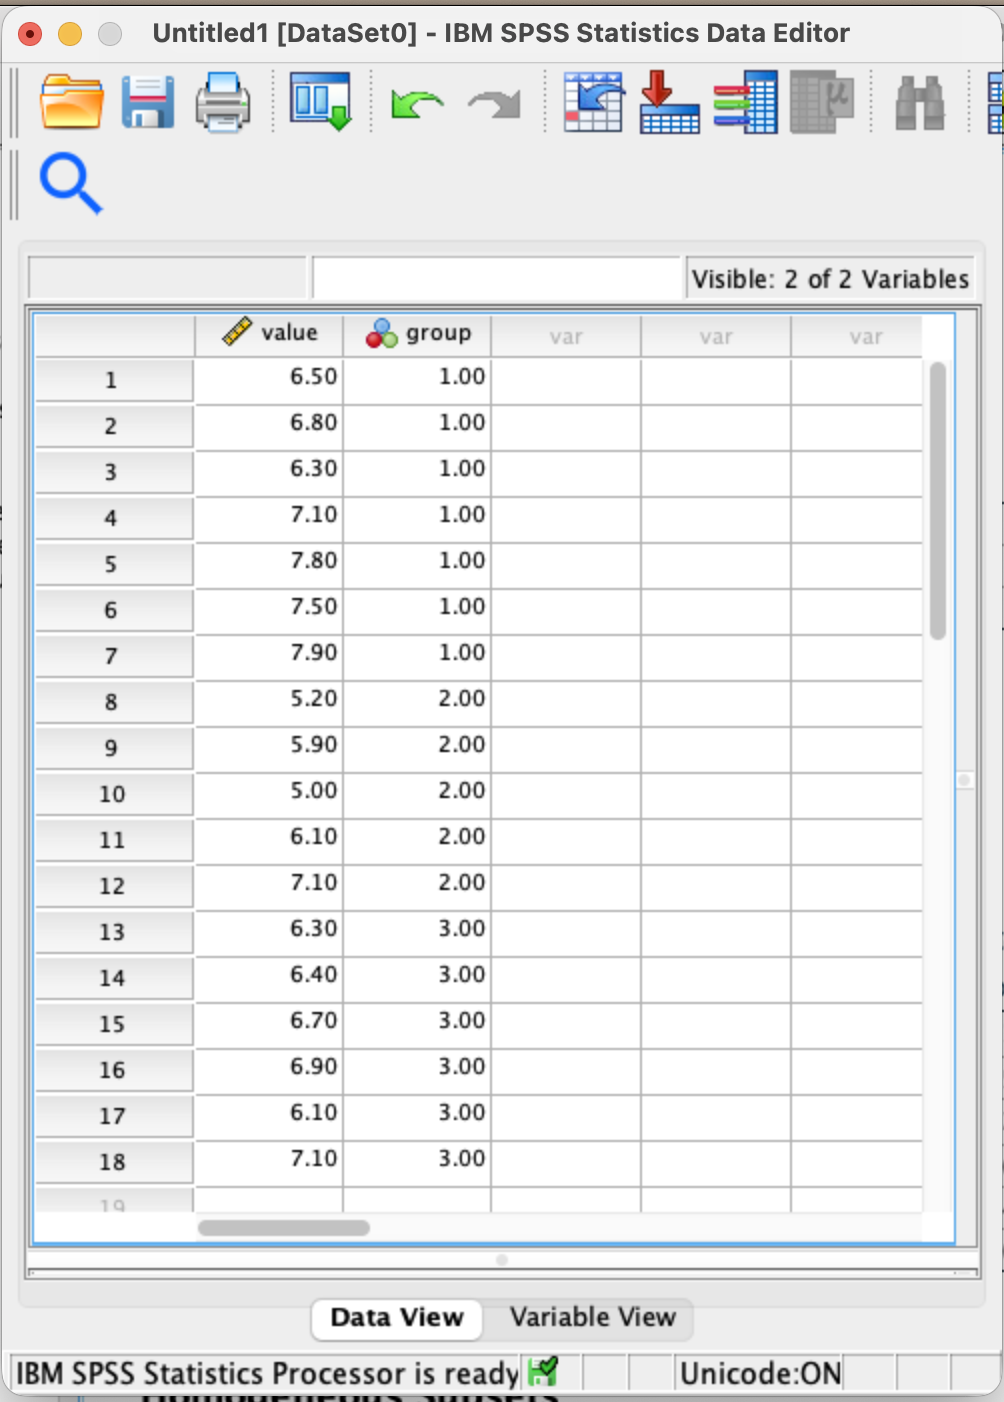
\includegraphics[width=0.5\textwidth]{LAB02/pics/spss_data.png}
    \caption{Nhập dữ liệu vào SPSS}
    \label{fig:spss_data}
\end{figure}

Trong cửa sổ \textbf{Variable View}, thiết lập:

\begin{itemize}
\item value: Type = Numeric, Measure = Scale
\item group: Type = Numeric, Measure = Nominal
\end{itemize}

\begin{figure}[!htp]
    \centering
    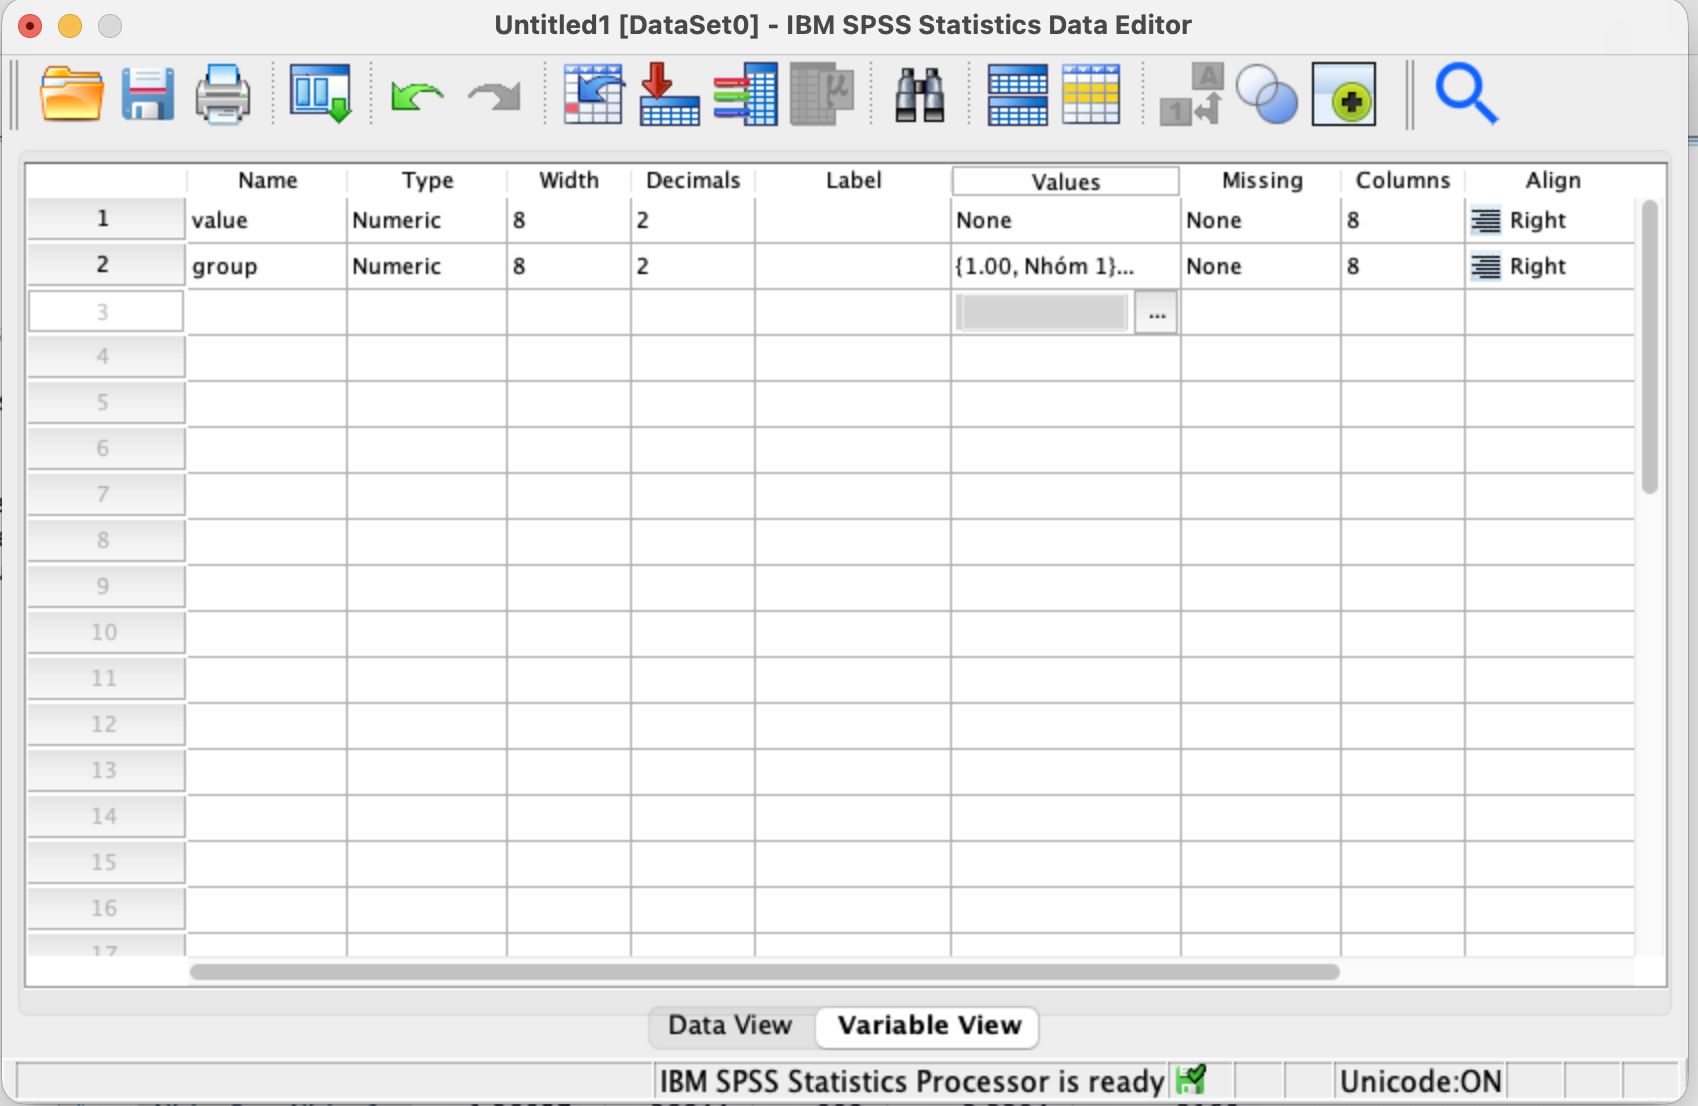
\includegraphics[width=0.8\textwidth]{LAB02/pics/spss_variables.png}
    \caption{Thiết lập các biến trong SPSS}
    \label{fig:spss_variable}
\end{figure}

\subsubsection*{Bước 2: Thực hiện phân tích One-way ANOVA}

Trên thanh menu của SPSS chọn:

\[
Analyze \rightarrow Compare\ Means \rightarrow One\text{-}Way\ ANOVA
\]

Sau đó chọn:

\begin{itemize}
\item \textbf{Dependent List}: value
\item \textbf{Factor}: group
\end{itemize}

\begin{figure}[!htp]
    \centering
    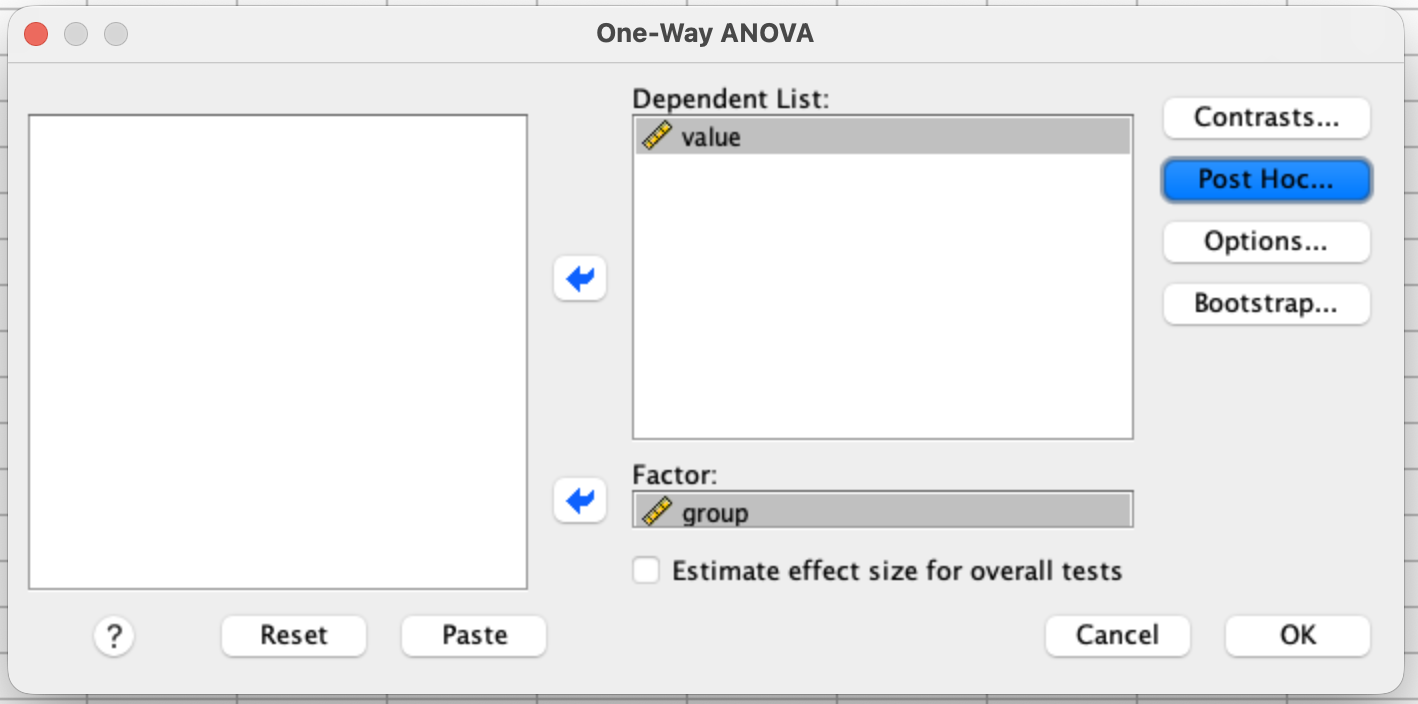
\includegraphics[width=0.8\textwidth]{LAB02/pics/spss_anova.png}
    \caption{Thiết lập phân tích One-way ANOVA}
    \label{fig:spss_anova}
\end{figure}

\subsubsection*{Bước 3: Thiết lập kiểm định Tukey}

Trong cửa sổ One-Way ANOVA (Hình \ref{fig:spss_anova}), nhấn \textbf{Post Hoc} và chọn phương pháp
\textbf{Tukey} với mức ý nghĩa $\alpha = 0.05$. (Hình \ref{fig:spss_tukey})

\begin{figure}[!htp]
    \centering
    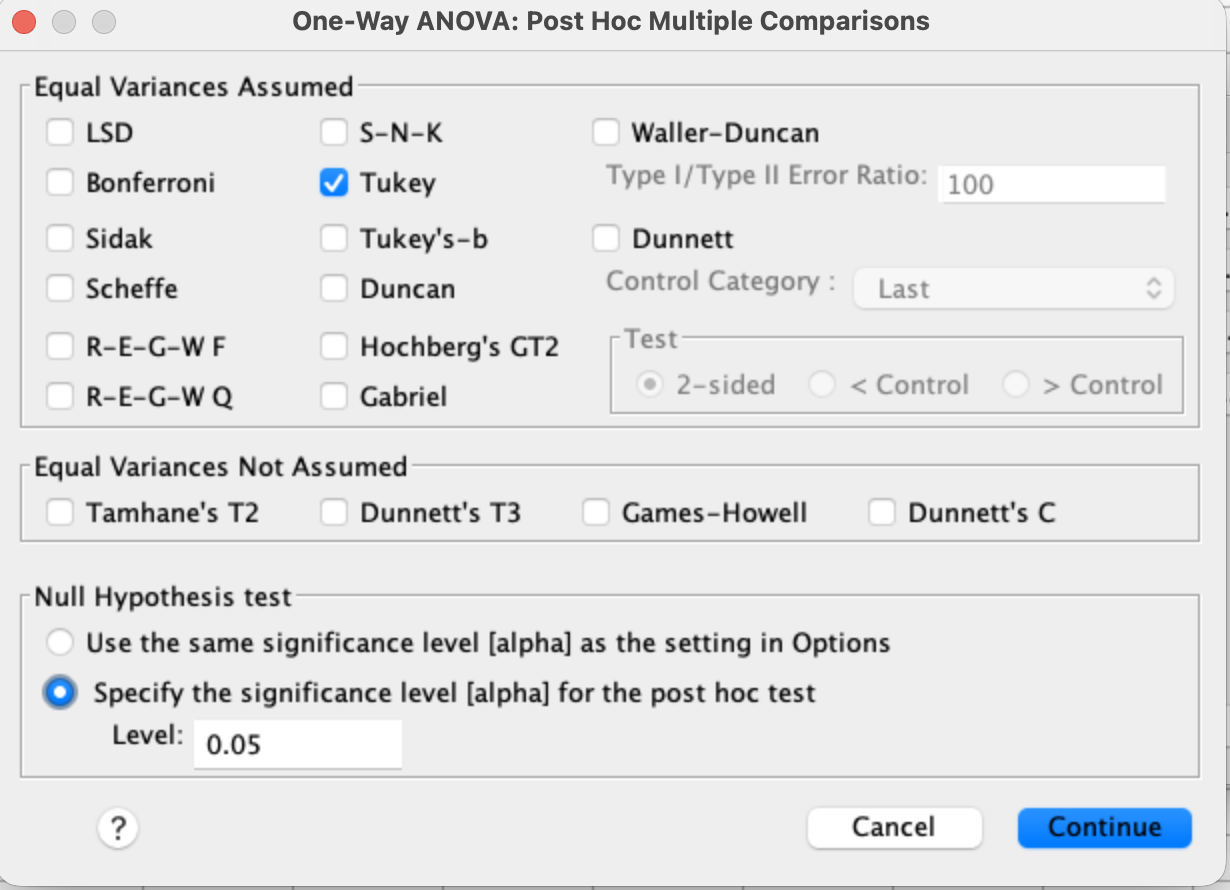
\includegraphics[width=0.8\textwidth]{LAB02/pics/spss_tukey.png}
    \caption{Thiết lập kiểm định hậu nghiệm Tukey HSD}
    \label{fig:spss_tukey}
\end{figure}

Sau đó nhấn \textbf{Continue} và chọn \textbf{OK} để chạy phân tích.

\subsubsection*{Bước 4: Kết quả ANOVA}

SPSS xuất bảng kết quả ANOVA như Hình \ref{fig:spss_result_anova}.

\begin{figure}[!htp]
    \centering
    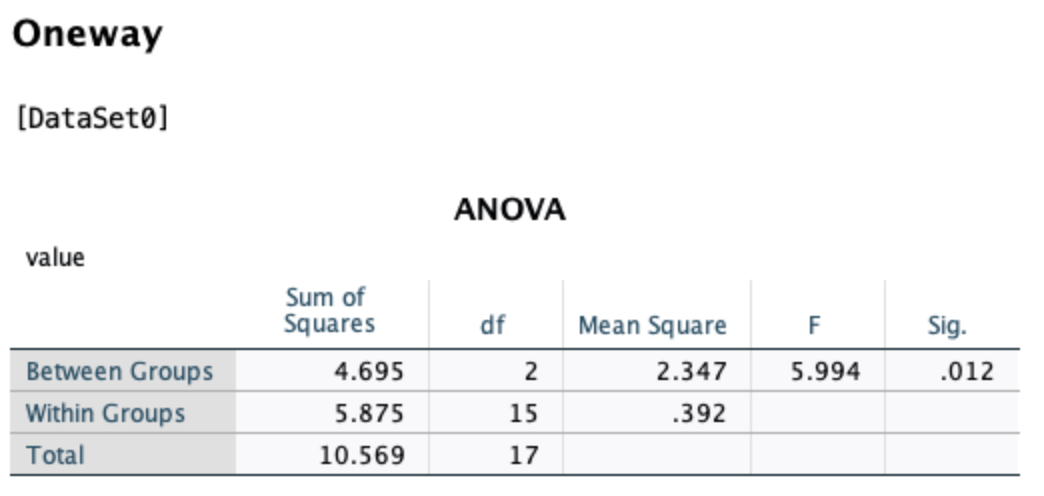
\includegraphics[width=0.8\textwidth]{LAB02/pics/spss_anova_result.png}
    \caption{Kết quả ANOVA trong SPSS}
    \label{fig:spss_result_anova}
\end{figure}

Từ kết quả ANOVA:

\[
F = 5.994, \quad p\text{-value} = 0.012
\]

Vì:

\[
p < 0.05
\]

nên bác bỏ giả thuyết $H_0$. Điều này cho thấy có sự khác biệt có ý nghĩa
thống kê giữa trung bình của ít nhất một cặp nhóm.

\subsubsection*{Bước 5: Kết quả kiểm định Tukey HSD}

Sau khi ANOVA cho kết quả có ý nghĩa thống kê, kiểm định hậu nghiệm
Tukey HSD được sử dụng để xác định cặp nhóm nào có sự khác biệt.

\begin{figure}[!htp]
    \centering
    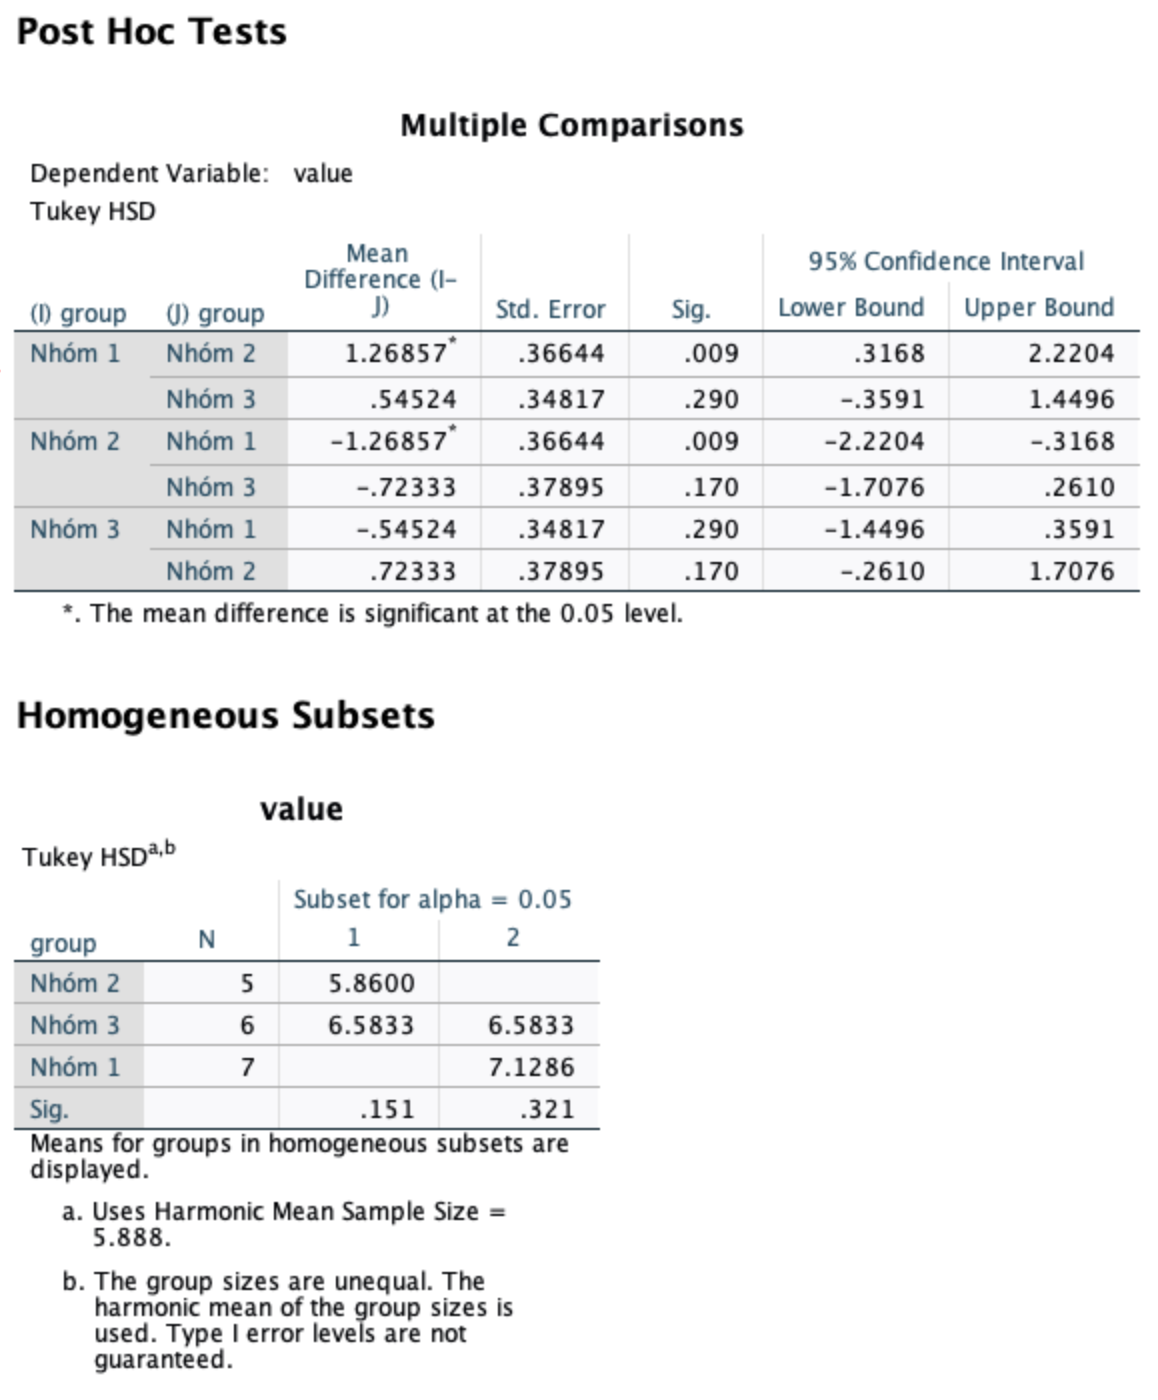
\includegraphics[width=0.8\textwidth]{LAB02/pics/spss_tukey_result.png}
    \caption{Kết quả kiểm định Tukey HSD}
    \label{fig:spss_tukey_result}
\end{figure}

Kết quả cho thấy:

\begin{itemize}
\item Nhóm 1 và Nhóm 2 có sự khác biệt có ý nghĩa thống kê (Sig = 0.009)
\item Nhóm 1 và Nhóm 3 không có sự khác biệt có ý nghĩa thống kê
\item Nhóm 2 và Nhóm 3 không có sự khác biệt có ý nghĩa thống kê
\end{itemize}

\subsubsection*{Bước 6: Diễn giải kết quả}

Từ kết quả kiểm định Tukey HSD, có thể kết luận rằng sự khác biệt trung bình
giữa các nhóm chủ yếu xuất hiện giữa \textbf{Nhóm 1 và Nhóm 2}.
Các cặp nhóm còn lại không có sự khác biệt đáng kể ở mức ý nghĩa $5\%$.

\subsection{Thực hiện phân tích One-way ANOVA và Tukey HSD bằng R}

Trong phần này, dữ liệu được phân tích bằng phần mềm R để kiểm tra
sự khác biệt trung bình giữa ba nhóm bằng phương pháp One-way ANOVA
và kiểm định hậu nghiệm Tukey HSD.

\subsubsection*{Bước 1: Nhập dữ liệu}

Dữ liệu được nhập vào R dưới dạng các vector:

\begin{verbatim}
group1 <- c(6.5,6.8,6.3,7.1,7.8,7.5,7.9)
group2 <- c(5.2,5.9,5,6.1,7.1)
group3 <- c(6.3,6.4,6.7,6.9,6.1,7.1)
\end{verbatim}

Sau đó tạo biến dữ liệu:

\begin{verbatim}
value <- c(group1, group2, group3)

group <- c(
rep("Nhom1",7),
rep("Nhom2",5),
rep("Nhom3",6)
)

data <- data.frame(value, group)
\end{verbatim}

\subsubsection*{Bước 2: Thực hiện One-way ANOVA}

Phân tích ANOVA được thực hiện bằng hàm:

\begin{verbatim}
anova_model <- aov(value ~ group, data = data)
summary(anova_model)
\end{verbatim}

Kết quả ANOVA được trình bày trong Bảng \ref{tab:r_anova}.

\begin{table}[!htp]
\centering
\caption{Kết quả ANOVA trong R}
\label{tab:r_anova}
\begin{tabular}{|c|c|c|c|c|}
\hline
Source & Df & Sum Sq & Mean Sq & F value \\
\hline
Group & 2 & 4.695 & 2.3474 & 5.994 \\
Residuals & 15 & 5.875 & 0.3916 & \\
\hline
\end{tabular}
\end{table}

Giá trị $p$-value thu được là:

\[
p = 0.0122
\]

Vì:

\[
p < 0.05
\]

nên bác bỏ giả thuyết $H_0$. Điều này cho thấy có sự khác biệt có ý nghĩa
thống kê giữa trung bình của ít nhất một cặp nhóm.

\subsubsection*{Bước 3: Kiểm định Tukey HSD}

Sau khi ANOVA cho kết quả có ý nghĩa thống kê, kiểm định hậu nghiệm
Tukey HSD được thực hiện bằng lệnh:

\begin{verbatim}
TukeyHSD(anova_model)
\end{verbatim}

Kết quả được trình bày trong Bảng \ref{tab:r_tukey}.

\begin{table}[!htp]
\centering
\caption{Kết quả kiểm định Tukey HSD trong R}
\label{tab:r_tukey}
\begin{tabular}{|c|c|c|c|c|}
\hline
Comparison & Mean diff & Lower CI & Upper CI & p-value \\
\hline
Nhom2 - Nhom1 & -1.2686 & -2.2204 & -0.3168 & 0.0092 \\
Nhom3 - Nhom1 & -0.5452 & -1.4496 & 0.3591 & 0.2901 \\
Nhom3 - Nhom2 & 0.7233 & -0.2610 & 1.7076 & 0.1704 \\
\hline
\end{tabular}
\end{table}

Kết quả cho thấy:

\begin{itemize}
\item Nhóm 1 và Nhóm 2 có sự khác biệt có ý nghĩa thống kê ($p < 0.05$)
\item Nhóm 1 và Nhóm 3 không có sự khác biệt có ý nghĩa thống kê
\item Nhóm 2 và Nhóm 3 không có sự khác biệt có ý nghĩa thống kê
\end{itemize}

\subsubsection*{Bước 4: Minh họa dữ liệu bằng Boxplot}

Để trực quan hóa dữ liệu, biểu đồ Boxplot được vẽ bằng lệnh:

\begin{verbatim}
boxplot(value ~ group,
data = data,
col = "lightblue",
main = "Boxplot of Groups",
xlab = "Group",
ylab = "Value")
\end{verbatim}

\begin{figure}[!htp]
\centering
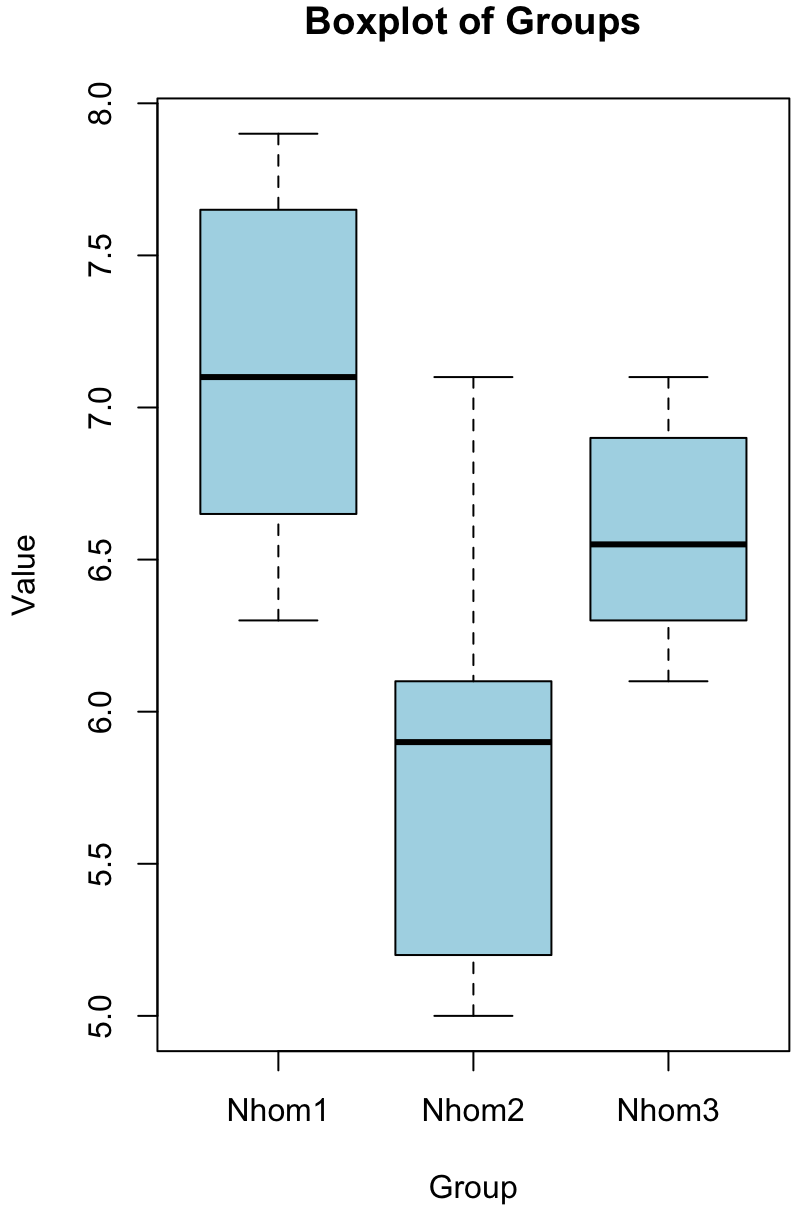
\includegraphics[width=0.5\textwidth]{LAB02/pics/r_boxplot.png}
\caption{Biểu đồ Boxplot của ba nhóm}
\label{fig:r_boxplot}
\end{figure}

\subsection{Thực hiện phân tích One-way ANOVA và Tukey HSD bằng Python}

Trong phần này, dữ liệu được phân tích bằng Python sử dụng các thư viện
\texttt{scipy} và \texttt{statsmodels} để thực hiện phân tích One-way ANOVA
và kiểm định hậu nghiệm Tukey HSD.

\subsubsection*{Bước 1: Nhập dữ liệu}

Dữ liệu được nhập vào Python dưới dạng các danh sách:

\begin{verbatim}
group1 = [6.5,6.8,6.3,7.1,7.8,7.5,7.9]
group2 = [5.2,5.9,5,6.1,7.1]
group3 = [6.3,6.4,6.7,6.9,6.1,7.1]
\end{verbatim}

\subsubsection*{Bước 2: Thực hiện One-way ANOVA}

Phân tích ANOVA được thực hiện bằng hàm:

\begin{verbatim}
stats.f_oneway(group1, group2, group3)
\end{verbatim}

Kết quả thu được:

\[
F = 5.9938
\]

\[
p = 0.0122
\]

Vì:

\[
p < 0.05
\]

nên bác bỏ giả thuyết $H_0$. Điều này cho thấy có sự khác biệt có ý nghĩa
thống kê giữa trung bình của ít nhất một cặp nhóm.

\subsubsection*{Bước 3: Kiểm định Tukey HSD}

Sau khi ANOVA cho kết quả có ý nghĩa thống kê, kiểm định hậu nghiệm
Tukey HSD được thực hiện bằng thư viện \texttt{statsmodels}.

\begin{verbatim}
tukey = pairwise_tukeyhsd(data, groups, alpha=0.05)
print(tukey)
\end{verbatim}

Kết quả được trình bày trong Bảng \ref{tab:python_tukey}.

\begin{table}[!htp]
\centering
\caption{Kết quả kiểm định Tukey HSD trong Python}
\label{tab:python_tukey}
\begin{tabular}{|c|c|c|c|c|}
\hline
Comparison & Mean diff & Lower CI & Upper CI & Reject $H_0$ \\
\hline
Nhom1 - Nhom2 & -1.2686 & -2.2204 & -0.3168 & True \\
Nhom1 - Nhom3 & -0.5452 & -1.4496 & 0.3591 & False \\
Nhom2 - Nhom3 & 0.7233 & -0.2610 & 1.7076 & False \\
\hline
\end{tabular}
\end{table}

Kết quả cho thấy:

\begin{itemize}
\item Nhóm 1 và Nhóm 2 có sự khác biệt có ý nghĩa thống kê
\item Nhóm 1 và Nhóm 3 không có sự khác biệt có ý nghĩa thống kê
\item Nhóm 2 và Nhóm 3 không có sự khác biệt có ý nghĩa thống kê
\end{itemize}

\subsubsection*{Bước 4: Minh họa dữ liệu bằng Boxplot}

Để trực quan hóa dữ liệu, biểu đồ Boxplot được vẽ bằng thư viện
\texttt{matplotlib}.

\begin{verbatim}
plt.boxplot([group1,group2,group3],
labels=["Nhom1","Nhom2","Nhom3"])
plt.title("Boxplot of Groups")
plt.xlabel("Group")
plt.ylabel("Value")
plt.show()
\end{verbatim}

\begin{figure}[!htp]
\centering
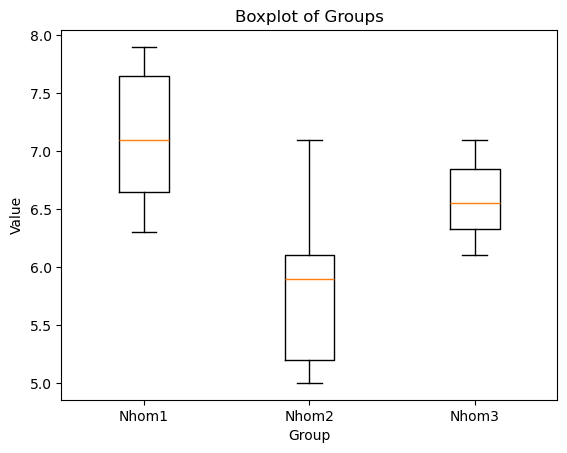
\includegraphics[width=0.7\textwidth]{LAB02/pics/python_boxplot.png}
\caption{Biểu đồ Boxplot của ba nhóm trong Python}
\label{fig:python_boxplot}
\end{figure}

\subsection{Nhận xét}

Kết quả phân tích dữ liệu bằng bốn công cụ khác nhau bao gồm
Excel, SPSS, R và Python đều cho kết quả tương đồng.

Cụ thể, giá trị $p$-value thu được từ các công cụ như sau:

\begin{table}[!htp]
\centering
\begin{tabular}{|c|c|}
\hline
\textbf{Công cụ} & \textbf{$p$-value} \\
\hline
Excel & 0.0122 \\
SPSS & 0.012 \\
R & 0.0122 \\
Python & 0.0122 \\
\hline
\end{tabular}
\caption{So sánh kết quả ANOVA giữa các công cụ}
\end{table}

Ta thấy rằng tất cả các công cụ đều cho $p$-value nhỏ hơn mức ý nghĩa
$\alpha = 0.05$. Do đó, giả thuyết $H_0$ bị bác bỏ.

Điều này cho thấy có sự khác biệt có ý nghĩa thống kê giữa trung bình
của ít nhất một cặp nhóm.

Ngoài ra, kết quả kiểm định hậu nghiệm Tukey HSD từ các công cụ
cũng cho thấy rằng sự khác biệt chủ yếu xảy ra giữa
\textbf{Nhóm 1 và Nhóm 2}, trong khi các cặp nhóm còn lại
không có sự khác biệt có ý nghĩa thống kê.

Việc thu được kết quả giống nhau từ nhiều công cụ phân tích
khác nhau cho thấy tính nhất quán và độ tin cậy của kết quả phân tích.

Như vậy, có thể khẳng định rằng phương pháp phân tích One-way ANOVA
và kiểm định Tukey HSD đã được thực hiện chính xác và cho kết quả
nhất quán trên nhiều phần mềm thống kê khác nhau.


\subsection{Phân tích Chi-square test}

Trong phần này, kiểm định Chi-square được sử dụng để kiểm tra xem
có sự liên quan giữa \textbf{giới tính (GIOITINH)} và
\textbf{trình độ học vấn (BANGCAP)} của 100 người tại TP.HCM hay không.

\subsubsection{Giả thuyết kiểm định}

\begin{itemize}
\item $H_0$: Không có mối liên hệ giữa giới tính và trình độ học vấn
\item $H_1$: Có mối liên hệ giữa giới tính và trình độ học vấn
\end{itemize}

\subsubsection{Bảng tần số chéo}

Bảng tần số chéo giữa hai biến GIOITINH và BANGCAP được thể hiện
trong Hình \ref{fig:chisquare_crosstab}.

\begin{figure}[!htp]
    \centering
    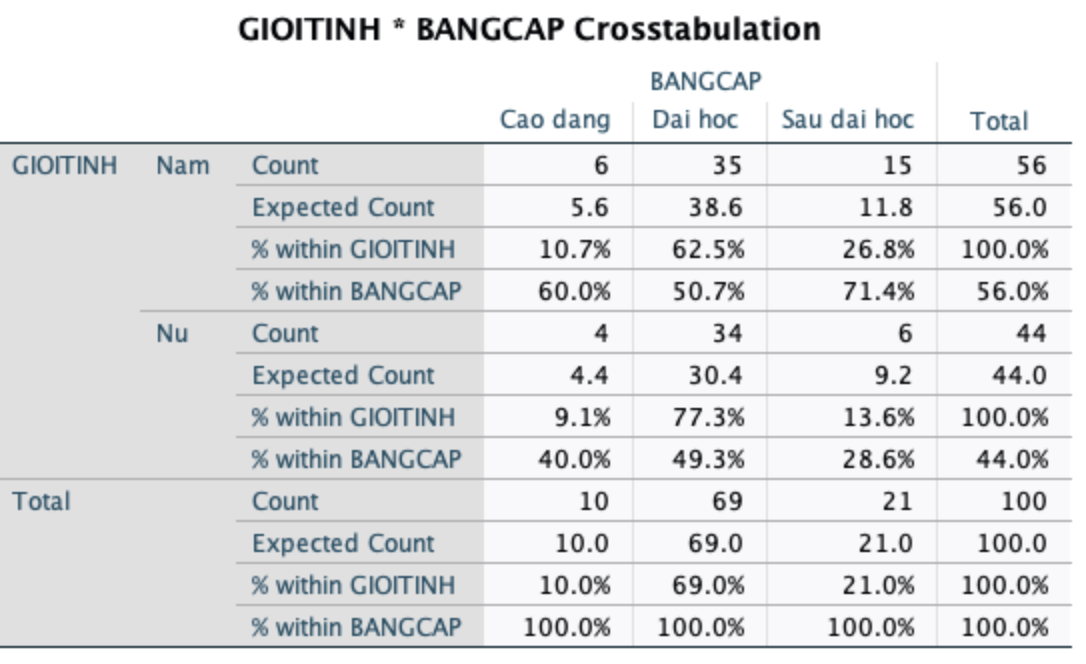
\includegraphics[width=0.85\textwidth]{LAB02/pics/chisquare_crosstab.png}
    \caption{Bảng Crosstab giữa GIOITINH và BANGCAP}
    \label{fig:chisquare_crosstab}
\end{figure}

Từ bảng trên ta có thể quan sát:

\begin{itemize}
\item Nam: 6 người cao đẳng, 35 người đại học, 15 người sau đại học
\item Nữ: 4 người cao đẳng, 34 người đại học, 6 người sau đại học
\end{itemize}

\subsubsection{Kết quả kiểm định Chi-square}

Kết quả kiểm định Chi-square được trình bày trong
Hình \ref{fig:chisquare_test}.

\begin{figure}[!htp]
    \centering
    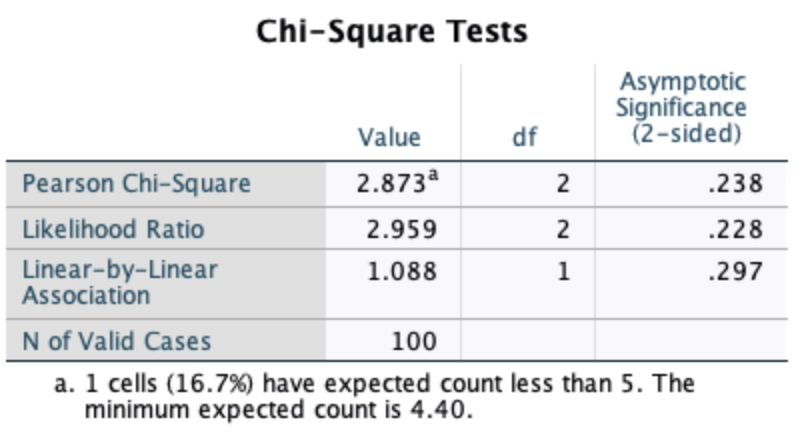
\includegraphics[width=0.6\textwidth]{LAB02/pics/chisquare_test.png}
    \caption{Kết quả kiểm định Chi-square}
    \label{fig:chisquare_test}
\end{figure}

Giá trị thống kê Pearson Chi-square:

\[
\chi^2 = 2.873
\]

Bậc tự do:

\[
df = 2
\]

Giá trị $p$-value:

\[
p = 0.238
\]

\subsubsection{Kết luận}

So sánh với mức ý nghĩa $\alpha = 0.05$:

\[
p = 0.238 > 0.05
\]

Do đó \textbf{không bác bỏ giả thuyết $H_0$}.

Điều này cho thấy \textbf{không có bằng chứng thống kê cho thấy
giới tính và trình độ học vấn có mối liên hệ với nhau}.
Nói cách khác, hai biến này được xem là \textbf{độc lập} trong
tập dữ liệu khảo sát 100 người tại TP.HCM.